Vào năm 1905, Albert Einstein đã công bố thuyết tương đối đặc biệt\footnote{Special Relativity (SR): Thuyết tương đối đặc biệt. Một số tài liệu dịch thành ``thuyết tương đối hẹp''.}. Thuyết tương đối đặc biệt dựa trên hai tiên đề:
\begin{itemize}
    \item Các định luật vật lý có cùng dạng trong mọi hệ quy chiếu quán tính.
    \item Tốc độ ánh sáng trong chân không là như nhau đối với mọi hệ quy chiếu quán tính.
\end{itemize}
Thuyết tương đối đặc biệt dẫn đến ba hệ quả quan trọng: sự mất tính đồng thời, giãn nở thời gian và co ngắn độ dài khi một vật thể chuyển động với vận tốc tiệm cận vận tốc ánh sáng. Năm 1908, Hermann Minkowski đã giới thiệu một cách diễn giải hình học của thuyết tương đối đặc biệt bằng khái niệm không--thời gian bốn chiều. Trong bài toán này, ta sẽ tìm hiểu về giản đồ Minkowski.

\vspace{8pt}

\subsection*{Giản đồ Minkowski}

\textbf{Không--thời gian Minkowski} là một mô hình hình học trong đó không gian và thời gian được gộp chung thành một hệ tọa độ thống nhất để mô tả các sự kiện và chuyển động trong thuyết tương đối đặc biệt. Quan hệ nhân quả giữa các sự kiện nằm trong nón ánh sáng không phụ thuộc vào hệ quy chiếu.\footnote{Trong khuôn khổ bài toán này, ta sử dụng cách mô tả trực quan.}

\vspace{8pt}

\textbf{Giản đồ Minkowski} biểu diễn các sự kiện trên một mặt phẳng với trục hoành \(x\) (mét) và trục tung \(ct\) (mét). Một điểm bất kỳ là \textbf{điểm thế giới} (world point), còn \textbf{đường thế giới} (worldline) là tập hợp các điểm thế giới biểu diễn chuyển động theo thời gian. Khi thay đổi hệ quy chiếu quán tính, các trục tọa độ ``xoay'' theo phép biến đổi hyperbol, trong khi các đường ánh sáng giữ nguyên phương.

\begin{figure}[h!]
\centering
\begin{figure}[!ht]
    \centering
    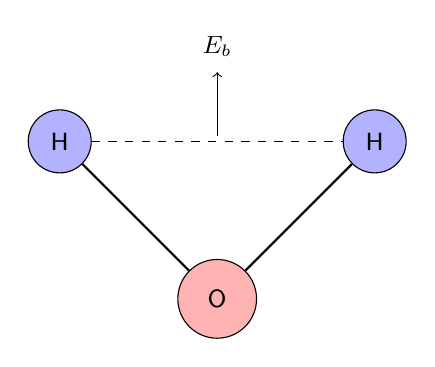
\begin{tikzpicture}[scale=2, font=\sansmath\sffamily, every node/.style={font=\sansmath\sffamily\small}]

% Nguyên tử Oxy
\node[circle, draw, fill=red!30, minimum size=1cm] (O) at (0,0) {O};

% Nguyên tử Hydro
\node[circle, draw, fill=blue!30, minimum size=0.8cm] (H1) at (-1,1) {H};
\node[circle, draw, fill=blue!30, minimum size=0.8cm] (H2) at (1,1) {H};

% Các liên kết
\draw[thick] (O) -- (H1);
\draw[thick] (O) -- (H2);

% Đường gạch giữa hai nguyên tử Hydro
\draw[dashed] (H1) -- (H2);

% Ghi chú E_b
\node (Eb) at (0,1.6) {$E_b$};

% Mũi tên nhỏ từ đường gạch lên E_b
\draw[->, shorten >=2pt, shorten <=2pt] (0,1) -- (Eb);

\end{tikzpicture}
    \caption{Lực liên kết}
\end{figure}

\caption{Sự thay đổi của các trục tọa độ khi chuyển hệ quy chiếu}
\end{figure}

\textbf{Nón ánh sáng} (light cone) của một sự kiện được xác định bởi các đường ánh sáng xuất phát từ sự kiện đó. Chia không--thời gian thành ba miền:
\begin{itemize}
    \item Miền tương lai và quá khứ: \(s^2>0\), gồm các sự kiện có thể có quan hệ nhân quả.
    \item Miền không gian (spacelike): \(s^2<0\), gồm các sự kiện \textbf{không thể} có quan hệ nhân quả.
    \item Đường ánh sáng: \(s^2=0\),
\end{itemize}
trong đó \(s^2\) đặc trưng quan hệ nhân quả giữa hai sự kiện.

\vspace{8pt}

1. Xây dựng biểu thức bất biến:
\[
s^2 = c^2 t^2 - x^2
\]
biết rằng \(s^2\) bất biến trong mọi hệ quy chiếu quán tính.

\emph{Gợi ý:} Tìm đại lượng \(f(t,x)\) bằng 0 cho ánh sáng truyền theo cả hai chiều \(\pm x\).
\vspace{8pt}

2. Bằng giản đồ Minkowski, chỉ ra rằng nếu tồn tại tín hiệu nhanh hơn ánh sáng, tính nhân quả sẽ bị vi phạm. Giải thích vì sao tốc độ ánh sáng đóng vai trò ``giới hạn tốc độ''.
\vspace{8pt}

3. Tìm hệ số hiệu chỉnh khi chuyển đơn vị trên các trục nghiêng \(x', ct'\) trong giản đồ Minkowski (dùng khi vẽ Minkowski bằng hình học Euclid).
\vspace{8pt}

\subsection*{Hành tinh \(P\) xấu số}

Xét hệ quy chiếu quán tính \(M\) gắn với hành tinh \(P\). Trên trục \(x\) (mét) có hai ngôi sao \(A\) và \(B\) nằm cùng phía so với \(P\), với tọa độ:
\[
x_A = a, \quad x_B = 2a.
\] 
Trong hệ \(M\), hai ngôi sao phát nổ đồng thời tại thời điểm \(t = t_0\) (giây). Tại \(t=0\), tàu vũ trụ \textit{Milky} rời \(P\) và chuyển động dọc trục \(x\) với vận tốc không đổi \(v = kc\), \(0<k<1\).

4. Bằng giản đồ Minkowski, tính thời gian riêng \(\tau\) của tàu giữa hai sự kiện:
\[
E_0: (t=0, x=0): \text{tàu rời } P
\]
\[
E_1: (t = \frac{a}{v}, x=a): \text{tàu đi qua vị trí ngôi sao } A
\]

\emph{Áp dụng số:} \(k=0.7, a=300\,\mathrm{AU}\) (1 AU = \(1.496\times10^{11}\) m).
\vspace{8pt}

5. Xác định độ lệch tọa độ thời gian giữa hai sự kiện nổ của các ngôi sao khi quan sát từ hệ quy chiếu gắn với tàu \textit{Milky}.
\vspace{8pt}

\begin{flushright}
    (biên soạn bởi Carina và KhorzX)
\end{flushright}